 \documentclass{article}
\usepackage[utf8]{inputenc}
\usepackage[a4paper, total={7in, 10in}]{geometry}
\usepackage{braket}
\usepackage{xcolor}
\usepackage{amsmath}
\usepackage{amssymb}
\usepackage{amsfonts}
\usepackage{graphicx}
\usepackage{svg}
\usepackage{float}
\usepackage{tikz}
\usepackage[ruled,vlined]{algorithm2e}
\usepackage{multicol}
\usepackage[backend=biber,style=alphabetic,sorting=ynt]{biblatex}
\usepackage{xcolor}
%\addbibresource{sample.bib} %Import the bibliography file

\newcommand{\commentt}[1]{\textcolor{blue}{ \textbf{[COMMENT]} #1}}
\newcommand{\ctt}[1]{\commentt{#1}}
\newcommand{\prb}[1]{ \mathbf{Pr} \left[ {#1} \right]}
\newcommand{\onotation}[1]{\(\mathcal{O} \left( {#1}  \right) \)}
\newcommand{\ona}[1]{\onotation{#1}}
\newcommand{\PSI}{{\ket{\psi}}}
\newcommand{\LESn}{\ket{\psi_n}}
\newcommand{\LESa}{\ket{\phi_n}}
\newcommand{\LESs}{\frac{1}{\sqrt{n}}\sum_{i}{\ket{\left(0^{i}10^{n-i}\right)^{n}}}}
\newcommand{\Hn}{\mathcal{H}_{n}}
\newcommand{\Ep}{\frac{1}{\sqrt{2^n}}\sum^{2^n}_{x}{ \ket{xx}}}
\newcommand{\HON}{\ket{\psi_{\text{honest}}}}
\newcommand{\Lemma}{\paragraph{Lemma.}}


\setlength{\columnsep}{0.6cm}

\newcommand{\Gz}{ G_{z}^{\delta} } 

\begin{document}

\title{Quantum LTC With Positive Rate}
\author{David Ponarovsky}
\maketitle
%\begin{multicols*}{2}
\newcommand{ \Hw }{ \delta\Delta -\Delta^{\frac{1}{2}-\varepsilon}/\delta  }
	\newcommand{ \Nw }{ \Delta^{\frac{3}{2}-\varepsilon}} 
	  \newcommand{ \Gu } { \Gamma^{\cup} }
	  \newcommand{ \Guq } { \Gamma^{\cup, \square} }

    	\newcommand{ \Gsa } {\Gamma_{\square_{1}} }
	\newcommand{ \Gsb } {\Gamma_{\square_{2}} }
        \newcommand{ \Aa } { C_{A_{1}}}  
	\newcommand{ \Ab } { C_{A_{2}}}
	\newcommand{ \Ac } { C_{A_{3}}}
	\newcommand{ \Aab } { \Aa \otimes \Ab } 
	\newcommand{ \Aac } { \Aa \otimes \Ac }
	\newcommand{ \Aabc } { \Aa \otimes \Ab \otimes \Ac }
	\newcommand{ \Aabp } { \Aa^{\perp} \otimes \Ab^{\perp} } 
	\newcommand{ \Aacp } { \Aa^{\perp} \otimes \Ac^{\perp} }
	\newcommand{ \Aabcp } { \Aa^{\perp} \otimes \Ab^{\perp} \otimes \Ac^{\perp} }
	\newcommand{ \Aabpp } { \left( \Aabp \right)^\perp } 
	\newcommand{ \Aacpp } { \left( \Aacp \right)^\perp }
	\newcommand{ \Aabcpp } { \left( \Aabcp \right)^\perp }
	\newcommand{ \YY } {  y_{1}y_{2}^{\top} }
	\newcommand{ \ZZ } {  z_{1}z_{2}^{\top} } 
	\newcommand{ \TT } { \tilde{\tau} } 


  \paragraph{preamble.} preamble.  
  \begin{figure}[H]
            %\label{fig:square}
            \begin{center}
            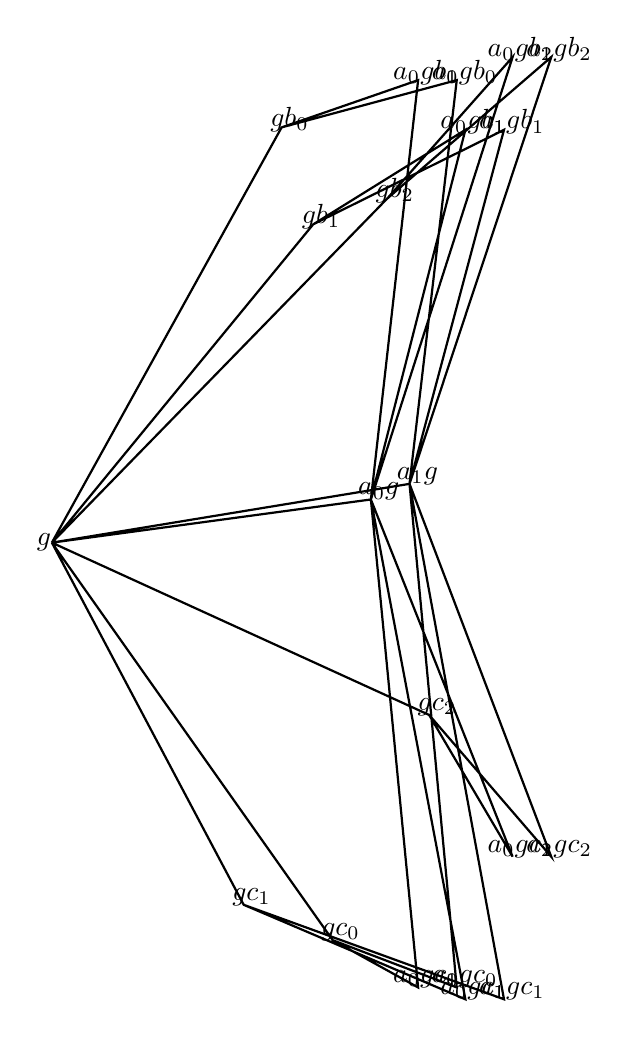
\begin{tikzpicture}
            \draw[thick](0,0)(0,0) -- (2.9181773873964936,5.273848202982883) -- (4.651477795555673,5.873848202982883) -- (4.051477795555673,0.5482605998168089) -- (0,0)
(0,0) -- (3.319058768389291,4.042603437245978) -- (5.251477795555673,5.242603437245978) -- (4.051477795555673,0.5482605998168089) -- (0,0)
(0,0) -- (4.256159121489313,4.366896433874894) -- (5.851477795555673,6.166896433874894) -- (4.051477795555673,0.5482605998168089) -- (0,0)
(0,0) -- (2.9181773873964936,5.273848202982883) -- (5.141960234544173,5.873848202982883) -- (4.541960234544173,0.7467321298508657) -- (0,0)
(0,0) -- (3.319058768389291,4.042603437245978) -- (5.741960234544173,5.242603437245978) -- (4.541960234544173,0.7467321298508657) -- (0,0)
(0,0) -- (4.256159121489313,4.366896433874894) -- (6.341960234544173,6.166896433874894) -- (4.541960234544173,0.7467321298508657) -- (0,0)
(0,0) -- (3.566636697886316,-5.048820087180208) -- (4.651477795555673,-5.648820087180208) -- (4.051477795555673,0.5482605998168089) -- (0,0)
(0,0) -- (2.436243474847646,-4.599078780926401) -- (5.251477795555673,-5.7990787809264015) -- (4.051477795555673,0.5482605998168089) -- (0,0)
(0,0) -- (4.791325381478329,-2.1881028354277494) -- (5.851477795555673,-3.9881028354277492) -- (4.051477795555673,0.5482605998168089) -- (0,0)
(0,0) -- (3.566636697886316,-5.048820087180208) -- (5.141960234544173,-5.648820087180208) -- (4.541960234544173,0.7467321298508657) -- (0,0)
(0,0) -- (2.436243474847646,-4.599078780926401) -- (5.741960234544173,-5.7990787809264015) -- (4.541960234544173,0.7467321298508657) -- (0,0)
(0,0) -- (4.791325381478329,-2.1881028354277494) -- (6.341960234544173,-3.9881028354277492) -- (4.541960234544173,0.7467321298508657) -- (0,0)
;
\node at (4.751477795555672,5.973848202982882) {$ a_{ 0  } gb_{ 0 } $};
\node at (5.351477795555673,5.342603437245978) {$ a_{ 0  } gb_{ 1 } $};
\node at (5.951477795555673,6.266896433874893) {$ a_{ 0  } gb_{ 2 } $};
\node at (5.241960234544172,5.973848202982882) {$ a_{ 1  } gb_{ 0 } $};
\node at (5.841960234544173,5.342603437245978) {$ a_{ 1  } gb_{ 1 } $};
\node at (6.441960234544172,6.266896433874893) {$ a_{ 1  } gb_{ 2 } $};
\node at (4.751477795555672,-5.548820087180208) {$ a_{ 0  } gc_{ 0 } $};
\node at (5.351477795555673,-5.699078780926402) {$ a_{ 0  } gc_{ 1 } $};
\node at (5.951477795555673,-3.888102835427749) {$ a_{ 0  } gc_{ 2 } $};
\node at (5.241960234544172,-5.548820087180208) {$ a_{ 1  } gc_{ 0 } $};
\node at (5.841960234544173,-5.699078780926402) {$ a_{ 1  } gc_{ 1 } $};
\node at (6.441960234544172,-3.888102835427749) {$ a_{ 1  } gc_{ 2 } $};
\node at (-0.1,0) {$ g $};
\node at (4.151477795555673,0.6482605998168088) {$ a_{ 0 }g $};
\node at (4.641960234544173,0.8467321298508657) {$ a_{ 1 }g $};
\node at (3.0181773873964937,5.373848202982883) {$ gb_{ 0 } $};
\node at (3.419058768389291,4.1426034372459775) {$ gb_{ 1 } $};
\node at (4.356159121489313,4.4668964338748935) {$ gb_{ 2 } $};
\node at (3.6666366978863163,-4.948820087180208) {$ gc_{ 0 } $};
\node at (2.536243474847646,-4.499078780926402) {$ gc_{ 1 } $};
\node at (4.891325381478329,-2.0881028354277493) {$ gc_{ 2 } $};

            \end{tikzpicture}
            \end{center}
            \caption{Square of the complex, with edges $(g,ag), (agb, gb) \in E_A,
            (g,gb), (agb, ag) \in E_B.$ \label{fig:square}
            }
            \end{figure}
 \begin{figure}[H]
            %\label{fig:square}
            \begin{center}
            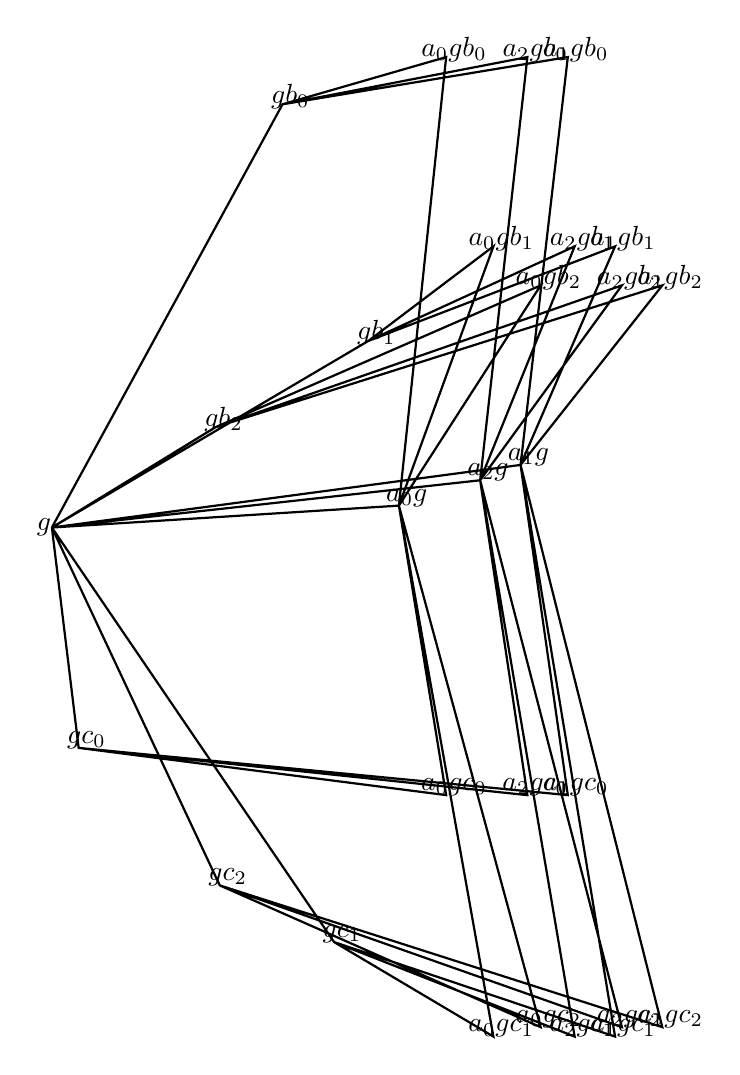
\begin{tikzpicture}
            \draw[thick](0,0)(0,0) -- (2.9295072406420357,5.374768980868401) -- (5.007356605656358,5.974768980868401) -- (4.407356605656358,0.27810190429716836) -- (0,0)
(0,0) -- (4.020516039047185,2.3704270907248945) -- (5.607356605656358,3.5704270907248947) -- (4.407356605656358,0.27810190429716836) -- (0,0)
(0,0) -- (2.0798965950067974,1.2749984961640073) -- (6.207356605656358,3.074998496164007) -- (4.407356605656358,0.27810190429716836) -- (0,0)
(0,0) -- (2.9295072406420357,5.374768980868401) -- (6.552522293629079,5.974768980868401) -- (5.952522293629079,0.7950658791584936) -- (0,0)
(0,0) -- (4.020516039047185,2.3704270907248945) -- (7.1525222936290795,3.5704270907248947) -- (5.952522293629079,0.7950658791584936) -- (0,0)
(0,0) -- (2.0798965950067974,1.2749984961640073) -- (7.752522293629079,3.074998496164007) -- (5.952522293629079,0.7950658791584936) -- (0,0)
(0,0) -- (2.9295072406420357,5.374768980868401) -- (6.039227674900031,5.974768980868401) -- (5.439227674900032,0.5999855228306958) -- (0,0)
(0,0) -- (4.020516039047185,2.3704270907248945) -- (6.639227674900032,3.5704270907248947) -- (5.439227674900032,0.5999855228306958) -- (0,0)
(0,0) -- (2.0798965950067974,1.2749984961640073) -- (7.2392276749000315,3.074998496164007) -- (5.439227674900032,0.5999855228306958) -- (0,0)
(0,0) -- (0.34016545974966783,-2.7985517909963904) -- (5.007356605656358,-3.3985517909963905) -- (4.407356605656358,0.27810190429716836) -- (0,0)
(0,0) -- (3.5844177259096788,-5.264863751096221) -- (5.607356605656358,-6.464863751096221) -- (4.407356605656358,0.27810190429716836) -- (0,0)
(0,0) -- (2.1325959362854414,-4.545131348462909) -- (6.207356605656358,-6.345131348462909) -- (4.407356605656358,0.27810190429716836) -- (0,0)
(0,0) -- (0.34016545974966783,-2.7985517909963904) -- (6.552522293629079,-3.3985517909963905) -- (5.952522293629079,0.7950658791584936) -- (0,0)
(0,0) -- (3.5844177259096788,-5.264863751096221) -- (7.1525222936290795,-6.464863751096221) -- (5.952522293629079,0.7950658791584936) -- (0,0)
(0,0) -- (2.1325959362854414,-4.545131348462909) -- (7.752522293629079,-6.345131348462909) -- (5.952522293629079,0.7950658791584936) -- (0,0)
(0,0) -- (0.34016545974966783,-2.7985517909963904) -- (6.039227674900031,-3.3985517909963905) -- (5.439227674900032,0.5999855228306958) -- (0,0)
(0,0) -- (3.5844177259096788,-5.264863751096221) -- (6.639227674900032,-6.464863751096221) -- (5.439227674900032,0.5999855228306958) -- (0,0)
(0,0) -- (2.1325959362854414,-4.545131348462909) -- (7.2392276749000315,-6.345131348462909) -- (5.439227674900032,0.5999855228306958) -- (0,0)
;
\node at (5.107356605656357,6.0747689808684004) {$ a_{ 0  } gb_{ 0 } $};
\node at (5.707356605656358,3.670427090724895) {$ a_{ 0  } gb_{ 1 } $};
\node at (6.3073566056563575,3.174998496164007) {$ a_{ 0  } gb_{ 2 } $};
\node at (6.652522293629079,6.0747689808684004) {$ a_{ 1  } gb_{ 0 } $};
\node at (7.252522293629079,3.670427090724895) {$ a_{ 1  } gb_{ 1 } $};
\node at (7.852522293629079,3.174998496164007) {$ a_{ 1  } gb_{ 2 } $};
\node at (6.139227674900031,6.0747689808684004) {$ a_{ 2  } gb_{ 0 } $};
\node at (6.7392276749000315,3.670427090724895) {$ a_{ 2  } gb_{ 1 } $};
\node at (7.339227674900031,3.174998496164007) {$ a_{ 2  } gb_{ 2 } $};
\node at (5.107356605656357,-3.2985517909963904) {$ a_{ 0  } gc_{ 0 } $};
\node at (5.707356605656358,-6.364863751096221) {$ a_{ 0  } gc_{ 1 } $};
\node at (6.3073566056563575,-6.245131348462909) {$ a_{ 0  } gc_{ 2 } $};
\node at (6.652522293629079,-3.2985517909963904) {$ a_{ 1  } gc_{ 0 } $};
\node at (7.252522293629079,-6.364863751096221) {$ a_{ 1  } gc_{ 1 } $};
\node at (7.852522293629079,-6.245131348462909) {$ a_{ 1  } gc_{ 2 } $};
\node at (6.139227674900031,-3.2985517909963904) {$ a_{ 2  } gc_{ 0 } $};
\node at (6.7392276749000315,-6.364863751096221) {$ a_{ 2  } gc_{ 1 } $};
\node at (7.339227674900031,-6.245131348462909) {$ a_{ 2  } gc_{ 2 } $};
\node at (-0.1,0) {$ g $};
\node at (4.507356605656358,0.3781019042971684) {$ a_{ 0 }g $};
\node at (6.052522293629079,0.8950658791584936) {$ a_{ 1 }g $};
\node at (5.539227674900031,0.6999855228306958) {$ a_{ 2 }g $};
\node at (3.029507240642036,5.474768980868401) {$ gb_{ 0 } $};
\node at (4.120516039047184,2.4704270907248946) {$ gb_{ 1 } $};
\node at (2.1798965950067974,1.3749984961640074) {$ gb_{ 2 } $};
\node at (0.4401654597496678,-2.6985517909963903) {$ gc_{ 0 } $};
\node at (3.684417725909679,-5.164863751096221) {$ gc_{ 1 } $};
\node at (2.2325959362854415,-4.445131348462909) {$ gc_{ 2 } $};

            \end{tikzpicture}
            \end{center}
            \caption{Square of the complex, with edges $(g,ag), (agb, gb) \in E_A,
            (g,gb), (agb, ag) \in E_B.$ \label{fig:square}
            }
            \end{figure}
 \begin{figure}[H]
            %\label{fig:square}
            \begin{center}
            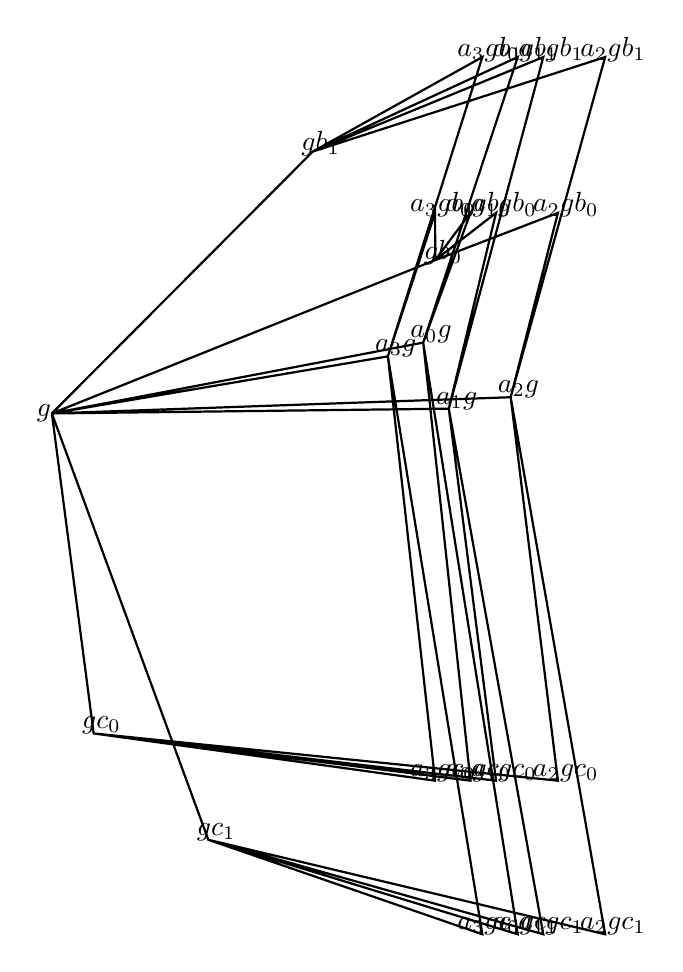
\begin{tikzpicture}
            \draw[thick](0,0)(0,0) -- (4.8678260761982015,1.947276727355456) -- (5.316102475267831,2.547276727355456) -- (4.7161024752678316,0.8993297857561124) -- (0,0)
(0,0) -- (3.313877154292573,3.3255864264278414) -- (5.916102475267832,4.525586426427841) -- (4.7161024752678316,0.8993297857561124) -- (0,0)
(0,0) -- (4.8678260761982015,1.947276727355456) -- (5.640968773917893,2.547276727355456) -- (5.040968773917894,0.05999360935056974) -- (0,0)
(0,0) -- (3.313877154292573,3.3255864264278414) -- (6.240968773917894,4.525586426427841) -- (5.040968773917894,0.05999360935056974) -- (0,0)
(0,0) -- (4.8678260761982015,1.947276727355456) -- (6.426688224410608,2.547276727355456) -- (5.826688224410608,0.20568042133633527) -- (0,0)
(0,0) -- (3.313877154292573,3.3255864264278414) -- (7.026688224410608,4.525586426427841) -- (5.826688224410608,0.20568042133633527) -- (0,0)
(0,0) -- (4.8678260761982015,1.947276727355456) -- (4.867245195881757,2.547276727355456) -- (4.267245195881757,0.7245984459213471) -- (0,0)
(0,0) -- (3.313877154292573,3.3255864264278414) -- (5.467245195881757,4.525586426427841) -- (4.267245195881757,0.7245984459213471) -- (0,0)
(0,0) -- (0.530779309698417,-4.064188879643348) -- (5.316102475267831,-4.664188879643348) -- (4.7161024752678316,0.8993297857561124) -- (0,0)
(0,0) -- (1.9871443633789636,-5.414744671117091) -- (5.916102475267832,-6.614744671117091) -- (4.7161024752678316,0.8993297857561124) -- (0,0)
(0,0) -- (0.530779309698417,-4.064188879643348) -- (5.640968773917893,-4.664188879643348) -- (5.040968773917894,0.05999360935056974) -- (0,0)
(0,0) -- (1.9871443633789636,-5.414744671117091) -- (6.240968773917894,-6.614744671117091) -- (5.040968773917894,0.05999360935056974) -- (0,0)
(0,0) -- (0.530779309698417,-4.064188879643348) -- (6.426688224410608,-4.664188879643348) -- (5.826688224410608,0.20568042133633527) -- (0,0)
(0,0) -- (1.9871443633789636,-5.414744671117091) -- (7.026688224410608,-6.614744671117091) -- (5.826688224410608,0.20568042133633527) -- (0,0)
(0,0) -- (0.530779309698417,-4.064188879643348) -- (4.867245195881757,-4.664188879643348) -- (4.267245195881757,0.7245984459213471) -- (0,0)
(0,0) -- (1.9871443633789636,-5.414744671117091) -- (5.467245195881757,-6.614744671117091) -- (4.267245195881757,0.7245984459213471) -- (0,0)
;
\node at (5.416102475267831,2.647276727355456) {$ a_{ 0  } gb_{ 0 } $};
\node at (6.016102475267831,4.625586426427841) {$ a_{ 0  } gb_{ 1 } $};
\node at (5.740968773917893,2.647276727355456) {$ a_{ 1  } gb_{ 0 } $};
\node at (6.3409687739178935,4.625586426427841) {$ a_{ 1  } gb_{ 1 } $};
\node at (6.5266882244106075,2.647276727355456) {$ a_{ 2  } gb_{ 0 } $};
\node at (7.126688224410608,4.625586426427841) {$ a_{ 2  } gb_{ 1 } $};
\node at (4.967245195881756,2.647276727355456) {$ a_{ 3  } gb_{ 0 } $};
\node at (5.567245195881757,4.625586426427841) {$ a_{ 3  } gb_{ 1 } $};
\node at (5.416102475267831,-4.564188879643348) {$ a_{ 0  } gc_{ 0 } $};
\node at (6.016102475267831,-6.514744671117091) {$ a_{ 0  } gc_{ 1 } $};
\node at (5.740968773917893,-4.564188879643348) {$ a_{ 1  } gc_{ 0 } $};
\node at (6.3409687739178935,-6.514744671117091) {$ a_{ 1  } gc_{ 1 } $};
\node at (6.5266882244106075,-4.564188879643348) {$ a_{ 2  } gc_{ 0 } $};
\node at (7.126688224410608,-6.514744671117091) {$ a_{ 2  } gc_{ 1 } $};
\node at (4.967245195881756,-4.564188879643348) {$ a_{ 3  } gc_{ 0 } $};
\node at (5.567245195881757,-6.514744671117091) {$ a_{ 3  } gc_{ 1 } $};
\node at (-0.1,0) {$ g $};
\node at (4.816102475267831,0.9993297857561124) {$ a_{ 0 }g $};
\node at (5.140968773917893,0.15999360935056975) {$ a_{ 1 }g $};
\node at (5.926688224410608,0.3056804213363353) {$ a_{ 2 }g $};
\node at (4.367245195881757,0.8245984459213471) {$ a_{ 3 }g $};
\node at (4.967826076198201,2.047276727355456) {$ gb_{ 0 } $};
\node at (3.413877154292573,3.4255864264278415) {$ gb_{ 1 } $};
\node at (0.630779309698417,-3.964188879643348) {$ gc_{ 0 } $};
\node at (2.0871443633789637,-5.314744671117091) {$ gc_{ 1 } $};

            \end{tikzpicture}
            \end{center}
            \caption{Square of the complex, with edges $(g,ag), (agb, gb) \in E_A,
            (g,gb), (agb, ag) \in E_B.$ \label{fig:square}
            }
            \end{figure}
 \begin{figure}[H]
            %\label{fig:square}
            \begin{center}
            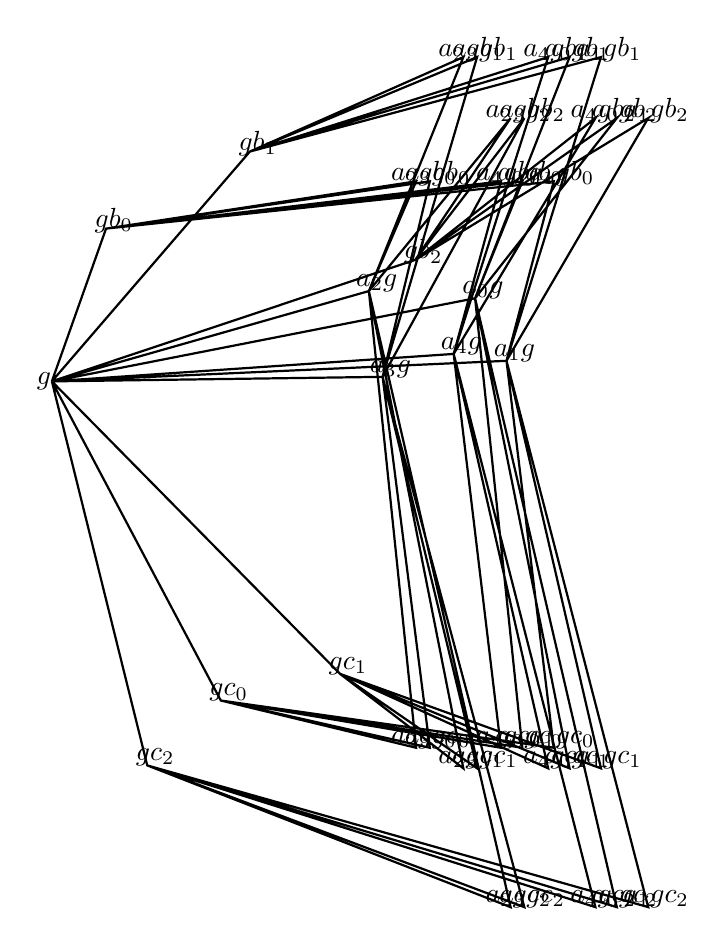
\begin{tikzpicture}
            \draw[thick](0,0)(0,0) -- (0.6881078757921377,1.9398994554271922) -- (5.974963879946981,2.539899455427192) -- (5.374963879946981,1.0553014401536618) -- (0,0)
(0,0) -- (2.514801418061513,2.9184028075189157) -- (6.574963879946981,4.118402807518915) -- (5.374963879946981,1.0553014401536618) -- (0,0)
(0,0) -- (4.61609878659953,1.543318022093987) -- (7.174963879946981,3.343318022093987) -- (5.374963879946981,1.0553014401536618) -- (0,0)
(0,0) -- (0.6881078757921377,1.9398994554271922) -- (6.373753694330703,2.539899455427192) -- (5.773753694330703,0.2608834492039341) -- (0,0)
(0,0) -- (2.514801418061513,2.9184028075189157) -- (6.9737536943307035,4.118402807518915) -- (5.773753694330703,0.2608834492039341) -- (0,0)
(0,0) -- (4.61609878659953,1.543318022093987) -- (7.573753694330703,3.343318022093987) -- (5.773753694330703,0.2608834492039341) -- (0,0)
(0,0) -- (0.6881078757921377,1.9398994554271922) -- (4.625964348724869,2.539899455427192) -- (4.0259643487248695,1.1466620954895166) -- (0,0)
(0,0) -- (2.514801418061513,2.9184028075189157) -- (5.22596434872487,4.118402807518915) -- (4.0259643487248695,1.1466620954895166) -- (0,0)
(0,0) -- (4.61609878659953,1.543318022093987) -- (5.825964348724869,3.343318022093987) -- (4.0259643487248695,1.1466620954895166) -- (0,0)
(0,0) -- (0.6881078757921377,1.9398994554271922) -- (4.80027795079803,2.539899455427192) -- (4.20027795079803,0.05717006630107852) -- (0,0)
(0,0) -- (2.514801418061513,2.9184028075189157) -- (5.4002779507980305,4.118402807518915) -- (4.20027795079803,0.05717006630107852) -- (0,0)
(0,0) -- (4.61609878659953,1.543318022093987) -- (6.00027795079803,3.343318022093987) -- (4.20027795079803,0.05717006630107852) -- (0,0)
(0,0) -- (0.6881078757921377,1.9398994554271922) -- (5.70300006395759,2.539899455427192) -- (5.10300006395759,0.34842054461517963) -- (0,0)
(0,0) -- (2.514801418061513,2.9184028075189157) -- (6.30300006395759,4.118402807518915) -- (5.10300006395759,0.34842054461517963) -- (0,0)
(0,0) -- (4.61609878659953,1.543318022093987) -- (6.90300006395759,3.343318022093987) -- (5.10300006395759,0.34842054461517963) -- (0,0)
(0,0) -- (2.1457268624869217,-4.053360593240427) -- (5.974963879946981,-4.653360593240427) -- (5.374963879946981,1.0553014401536618) -- (0,0)
(0,0) -- (3.6597096990926263,-3.714711325632788) -- (6.574963879946981,-4.914711325632788) -- (5.374963879946981,1.0553014401536618) -- (0,0)
(0,0) -- (1.2115213124479625,-4.877453669569164) -- (7.174963879946981,-6.6774536695691635) -- (5.374963879946981,1.0553014401536618) -- (0,0)
(0,0) -- (2.1457268624869217,-4.053360593240427) -- (6.373753694330703,-4.653360593240427) -- (5.773753694330703,0.2608834492039341) -- (0,0)
(0,0) -- (3.6597096990926263,-3.714711325632788) -- (6.9737536943307035,-4.914711325632788) -- (5.773753694330703,0.2608834492039341) -- (0,0)
(0,0) -- (1.2115213124479625,-4.877453669569164) -- (7.573753694330703,-6.6774536695691635) -- (5.773753694330703,0.2608834492039341) -- (0,0)
(0,0) -- (2.1457268624869217,-4.053360593240427) -- (4.625964348724869,-4.653360593240427) -- (4.0259643487248695,1.1466620954895166) -- (0,0)
(0,0) -- (3.6597096990926263,-3.714711325632788) -- (5.22596434872487,-4.914711325632788) -- (4.0259643487248695,1.1466620954895166) -- (0,0)
(0,0) -- (1.2115213124479625,-4.877453669569164) -- (5.825964348724869,-6.6774536695691635) -- (4.0259643487248695,1.1466620954895166) -- (0,0)
(0,0) -- (2.1457268624869217,-4.053360593240427) -- (4.80027795079803,-4.653360593240427) -- (4.20027795079803,0.05717006630107852) -- (0,0)
(0,0) -- (3.6597096990926263,-3.714711325632788) -- (5.4002779507980305,-4.914711325632788) -- (4.20027795079803,0.05717006630107852) -- (0,0)
(0,0) -- (1.2115213124479625,-4.877453669569164) -- (6.00027795079803,-6.6774536695691635) -- (4.20027795079803,0.05717006630107852) -- (0,0)
(0,0) -- (2.1457268624869217,-4.053360593240427) -- (5.70300006395759,-4.653360593240427) -- (5.10300006395759,0.34842054461517963) -- (0,0)
(0,0) -- (3.6597096990926263,-3.714711325632788) -- (6.30300006395759,-4.914711325632788) -- (5.10300006395759,0.34842054461517963) -- (0,0)
(0,0) -- (1.2115213124479625,-4.877453669569164) -- (6.90300006395759,-6.6774536695691635) -- (5.10300006395759,0.34842054461517963) -- (0,0)
;
\node at (6.0749638799469805,2.639899455427192) {$ a_{ 0  } gb_{ 0 } $};
\node at (6.674963879946981,4.218402807518915) {$ a_{ 0  } gb_{ 1 } $};
\node at (7.274963879946981,3.443318022093987) {$ a_{ 0  } gb_{ 2 } $};
\node at (6.473753694330703,2.639899455427192) {$ a_{ 1  } gb_{ 0 } $};
\node at (7.073753694330703,4.218402807518915) {$ a_{ 1  } gb_{ 1 } $};
\node at (7.673753694330703,3.443318022093987) {$ a_{ 1  } gb_{ 2 } $};
\node at (4.725964348724869,2.639899455427192) {$ a_{ 2  } gb_{ 0 } $};
\node at (5.325964348724869,4.218402807518915) {$ a_{ 2  } gb_{ 1 } $};
\node at (5.925964348724869,3.443318022093987) {$ a_{ 2  } gb_{ 2 } $};
\node at (4.90027795079803,2.639899455427192) {$ a_{ 3  } gb_{ 0 } $};
\node at (5.50027795079803,4.218402807518915) {$ a_{ 3  } gb_{ 1 } $};
\node at (6.10027795079803,3.443318022093987) {$ a_{ 3  } gb_{ 2 } $};
\node at (5.803000063957589,2.639899455427192) {$ a_{ 4  } gb_{ 0 } $};
\node at (6.40300006395759,4.218402807518915) {$ a_{ 4  } gb_{ 1 } $};
\node at (7.00300006395759,3.443318022093987) {$ a_{ 4  } gb_{ 2 } $};
\node at (6.0749638799469805,-4.553360593240427) {$ a_{ 0  } gc_{ 0 } $};
\node at (6.674963879946981,-4.814711325632788) {$ a_{ 0  } gc_{ 1 } $};
\node at (7.274963879946981,-6.577453669569164) {$ a_{ 0  } gc_{ 2 } $};
\node at (6.473753694330703,-4.553360593240427) {$ a_{ 1  } gc_{ 0 } $};
\node at (7.073753694330703,-4.814711325632788) {$ a_{ 1  } gc_{ 1 } $};
\node at (7.673753694330703,-6.577453669569164) {$ a_{ 1  } gc_{ 2 } $};
\node at (4.725964348724869,-4.553360593240427) {$ a_{ 2  } gc_{ 0 } $};
\node at (5.325964348724869,-4.814711325632788) {$ a_{ 2  } gc_{ 1 } $};
\node at (5.925964348724869,-6.577453669569164) {$ a_{ 2  } gc_{ 2 } $};
\node at (4.90027795079803,-4.553360593240427) {$ a_{ 3  } gc_{ 0 } $};
\node at (5.50027795079803,-4.814711325632788) {$ a_{ 3  } gc_{ 1 } $};
\node at (6.10027795079803,-6.577453669569164) {$ a_{ 3  } gc_{ 2 } $};
\node at (5.803000063957589,-4.553360593240427) {$ a_{ 4  } gc_{ 0 } $};
\node at (6.40300006395759,-4.814711325632788) {$ a_{ 4  } gc_{ 1 } $};
\node at (7.00300006395759,-6.577453669569164) {$ a_{ 4  } gc_{ 2 } $};
\node at (-0.1,0) {$ g $};
\node at (5.474963879946981,1.1553014401536619) {$ a_{ 0 }g $};
\node at (5.873753694330703,0.3608834492039341) {$ a_{ 1 }g $};
\node at (4.125964348724869,1.2466620954895167) {$ a_{ 2 }g $};
\node at (4.30027795079803,0.15717006630107852) {$ a_{ 3 }g $};
\node at (5.20300006395759,0.44842054461517966) {$ a_{ 4 }g $};
\node at (0.7881078757921377,2.039899455427192) {$ gb_{ 0 } $};
\node at (2.614801418061513,3.0184028075189158) {$ gb_{ 1 } $};
\node at (4.71609878659953,1.6433180220939871) {$ gb_{ 2 } $};
\node at (2.2457268624869218,-3.953360593240427) {$ gc_{ 0 } $};
\node at (3.7597096990926264,-3.614711325632788) {$ gc_{ 1 } $};
\node at (1.3115213124479626,-4.777453669569164) {$ gc_{ 2 } $};

            \end{tikzpicture}
            \end{center}
            \caption{Square of the complex, with edges $(g,ag), (agb, gb) \in E_A,
            (g,gb), (agb, ag) \in E_B.$ \label{fig:square}
            }
            \end{figure}
 \begin{figure}[H]
            %\label{fig:square}
            \begin{center}
            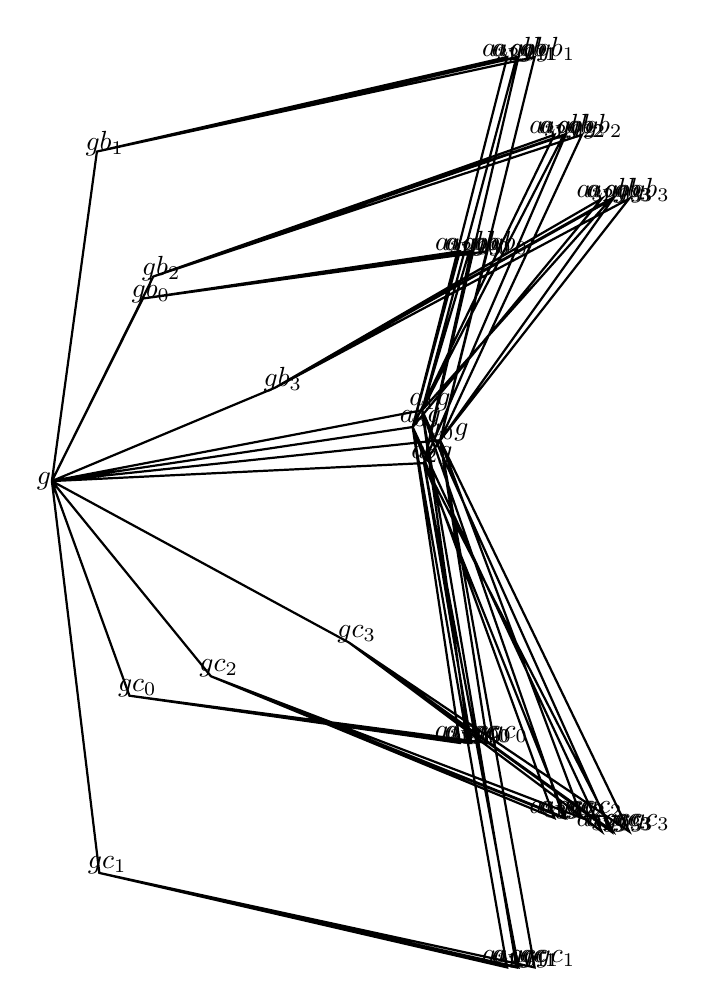
\begin{tikzpicture}
            \draw[thick](0,0)(0,0) -- (1.15688849512902,2.3185699842208587) -- (5.530732810575382,2.918569984220859) -- (4.930732810575383,0.51909139005912) -- (0,0)
(0,0) -- (0.5721458089845904,4.184921417501441) -- (6.130732810575383,5.384921417501441) -- (4.930732810575383,0.51909139005912) -- (0,0)
(0,0) -- (1.2889105286849474,2.598211411359821) -- (6.7307328105753825,4.398211411359821) -- (4.930732810575383,0.51909139005912) -- (0,0)
(0,0) -- (2.834221868558596,1.1859161884980924) -- (7.330732810575382,3.5859161884980923) -- (4.930732810575383,0.51909139005912) -- (0,0)
(0,0) -- (1.15688849512902,2.3185699842208587) -- (5.30139721439473,2.918569984220859) -- (4.7013972143947305,0.8994984517846364) -- (0,0)
(0,0) -- (0.5721458089845904,4.184921417501441) -- (5.901397214394731,5.384921417501441) -- (4.7013972143947305,0.8994984517846364) -- (0,0)
(0,0) -- (1.2889105286849474,2.598211411359821) -- (6.50139721439473,4.398211411359821) -- (4.7013972143947305,0.8994984517846364) -- (0,0)
(0,0) -- (2.834221868558596,1.1859161884980924) -- (7.10139721439473,3.5859161884980923) -- (4.7013972143947305,0.8994984517846364) -- (0,0)
(0,0) -- (1.15688849512902,2.3185699842208587) -- (5.326012475877157,2.918569984220859) -- (4.726012475877157,0.22830126075941862) -- (0,0)
(0,0) -- (0.5721458089845904,4.184921417501441) -- (5.926012475877157,5.384921417501441) -- (4.726012475877157,0.22830126075941862) -- (0,0)
(0,0) -- (1.2889105286849474,2.598211411359821) -- (6.526012475877157,4.398211411359821) -- (4.726012475877157,0.22830126075941862) -- (0,0)
(0,0) -- (2.834221868558596,1.1859161884980924) -- (7.1260124758771575,3.5859161884980923) -- (4.726012475877157,0.22830126075941862) -- (0,0)
(0,0) -- (1.15688849512902,2.3185699842208587) -- (5.181879568216868,2.918569984220859) -- (4.581879568216868,0.6864626546232614) -- (0,0)
(0,0) -- (0.5721458089845904,4.184921417501441) -- (5.781879568216868,5.384921417501441) -- (4.581879568216868,0.6864626546232614) -- (0,0)
(0,0) -- (1.2889105286849474,2.598211411359821) -- (6.381879568216868,4.398211411359821) -- (4.581879568216868,0.6864626546232614) -- (0,0)
(0,0) -- (2.834221868558596,1.1859161884980924) -- (6.981879568216868,3.5859161884980923) -- (4.581879568216868,0.6864626546232614) -- (0,0)
(0,0) -- (0.9855216424218832,-2.7256103515970174) -- (5.530732810575382,-3.3256103515970175) -- (4.930732810575383,0.51909139005912) -- (0,0)
(0,0) -- (0.6028754797563923,-4.976422889331044) -- (6.130732810575383,-6.176422889331044) -- (4.930732810575383,0.51909139005912) -- (0,0)
(0,0) -- (2.0198341676412417,-2.478736170197537) -- (6.7307328105753825,-4.278736170197536) -- (4.930732810575383,0.51909139005912) -- (0,0)
(0,0) -- (3.7716592879911865,-2.0494551613331926) -- (7.330732810575382,-4.4494551613331925) -- (4.930732810575383,0.51909139005912) -- (0,0)
(0,0) -- (0.9855216424218832,-2.7256103515970174) -- (5.30139721439473,-3.3256103515970175) -- (4.7013972143947305,0.8994984517846364) -- (0,0)
(0,0) -- (0.6028754797563923,-4.976422889331044) -- (5.901397214394731,-6.176422889331044) -- (4.7013972143947305,0.8994984517846364) -- (0,0)
(0,0) -- (2.0198341676412417,-2.478736170197537) -- (6.50139721439473,-4.278736170197536) -- (4.7013972143947305,0.8994984517846364) -- (0,0)
(0,0) -- (3.7716592879911865,-2.0494551613331926) -- (7.10139721439473,-4.4494551613331925) -- (4.7013972143947305,0.8994984517846364) -- (0,0)
(0,0) -- (0.9855216424218832,-2.7256103515970174) -- (5.326012475877157,-3.3256103515970175) -- (4.726012475877157,0.22830126075941862) -- (0,0)
(0,0) -- (0.6028754797563923,-4.976422889331044) -- (5.926012475877157,-6.176422889331044) -- (4.726012475877157,0.22830126075941862) -- (0,0)
(0,0) -- (2.0198341676412417,-2.478736170197537) -- (6.526012475877157,-4.278736170197536) -- (4.726012475877157,0.22830126075941862) -- (0,0)
(0,0) -- (3.7716592879911865,-2.0494551613331926) -- (7.1260124758771575,-4.4494551613331925) -- (4.726012475877157,0.22830126075941862) -- (0,0)
(0,0) -- (0.9855216424218832,-2.7256103515970174) -- (5.181879568216868,-3.3256103515970175) -- (4.581879568216868,0.6864626546232614) -- (0,0)
(0,0) -- (0.6028754797563923,-4.976422889331044) -- (5.781879568216868,-6.176422889331044) -- (4.581879568216868,0.6864626546232614) -- (0,0)
(0,0) -- (2.0198341676412417,-2.478736170197537) -- (6.381879568216868,-4.278736170197536) -- (4.581879568216868,0.6864626546232614) -- (0,0)
(0,0) -- (3.7716592879911865,-2.0494551613331926) -- (6.981879568216868,-4.4494551613331925) -- (4.581879568216868,0.6864626546232614) -- (0,0)
;
\node at (5.630732810575382,3.018569984220859) {$ a_{ 0  } gb_{ 0 } $};
\node at (6.2307328105753825,5.4849214175014405) {$ a_{ 0  } gb_{ 1 } $};
\node at (6.830732810575382,4.49821141135982) {$ a_{ 0  } gb_{ 2 } $};
\node at (7.430732810575382,3.6859161884980924) {$ a_{ 0  } gb_{ 3 } $};
\node at (5.40139721439473,3.018569984220859) {$ a_{ 1  } gb_{ 0 } $};
\node at (6.00139721439473,5.4849214175014405) {$ a_{ 1  } gb_{ 1 } $};
\node at (6.60139721439473,4.49821141135982) {$ a_{ 1  } gb_{ 2 } $};
\node at (7.20139721439473,3.6859161884980924) {$ a_{ 1  } gb_{ 3 } $};
\node at (5.426012475877156,3.018569984220859) {$ a_{ 2  } gb_{ 0 } $};
\node at (6.026012475877157,5.4849214175014405) {$ a_{ 2  } gb_{ 1 } $};
\node at (6.626012475877157,4.49821141135982) {$ a_{ 2  } gb_{ 2 } $};
\node at (7.226012475877157,3.6859161884980924) {$ a_{ 2  } gb_{ 3 } $};
\node at (5.281879568216867,3.018569984220859) {$ a_{ 3  } gb_{ 0 } $};
\node at (5.881879568216868,5.4849214175014405) {$ a_{ 3  } gb_{ 1 } $};
\node at (6.4818795682168675,4.49821141135982) {$ a_{ 3  } gb_{ 2 } $};
\node at (7.081879568216868,3.6859161884980924) {$ a_{ 3  } gb_{ 3 } $};
\node at (5.630732810575382,-3.2256103515970174) {$ a_{ 0  } gc_{ 0 } $};
\node at (6.2307328105753825,-6.076422889331044) {$ a_{ 0  } gc_{ 1 } $};
\node at (6.830732810575382,-4.178736170197537) {$ a_{ 0  } gc_{ 2 } $};
\node at (7.430732810575382,-4.349455161333193) {$ a_{ 0  } gc_{ 3 } $};
\node at (5.40139721439473,-3.2256103515970174) {$ a_{ 1  } gc_{ 0 } $};
\node at (6.00139721439473,-6.076422889331044) {$ a_{ 1  } gc_{ 1 } $};
\node at (6.60139721439473,-4.178736170197537) {$ a_{ 1  } gc_{ 2 } $};
\node at (7.20139721439473,-4.349455161333193) {$ a_{ 1  } gc_{ 3 } $};
\node at (5.426012475877156,-3.2256103515970174) {$ a_{ 2  } gc_{ 0 } $};
\node at (6.026012475877157,-6.076422889331044) {$ a_{ 2  } gc_{ 1 } $};
\node at (6.626012475877157,-4.178736170197537) {$ a_{ 2  } gc_{ 2 } $};
\node at (7.226012475877157,-4.349455161333193) {$ a_{ 2  } gc_{ 3 } $};
\node at (5.281879568216867,-3.2256103515970174) {$ a_{ 3  } gc_{ 0 } $};
\node at (5.881879568216868,-6.076422889331044) {$ a_{ 3  } gc_{ 1 } $};
\node at (6.4818795682168675,-4.178736170197537) {$ a_{ 3  } gc_{ 2 } $};
\node at (7.081879568216868,-4.349455161333193) {$ a_{ 3  } gc_{ 3 } $};
\node at (-0.1,0) {$ g $};
\node at (5.030732810575382,0.61909139005912) {$ a_{ 0 }g $};
\node at (4.80139721439473,0.9994984517846364) {$ a_{ 1 }g $};
\node at (4.826012475877157,0.3283012607594186) {$ a_{ 2 }g $};
\node at (4.681879568216868,0.7864626546232614) {$ a_{ 3 }g $};
\node at (1.25688849512902,2.418569984220859) {$ gb_{ 0 } $};
\node at (0.6721458089845904,4.28492141750144) {$ gb_{ 1 } $};
\node at (1.3889105286849475,2.698211411359821) {$ gb_{ 2 } $};
\node at (2.934221868558596,1.2859161884980925) {$ gb_{ 3 } $};
\node at (1.0855216424218832,-2.6256103515970173) {$ gc_{ 0 } $};
\node at (0.7028754797563923,-4.876422889331044) {$ gc_{ 1 } $};
\node at (2.1198341676412418,-2.378736170197537) {$ gc_{ 2 } $};
\node at (3.8716592879911866,-1.9494551613331925) {$ gc_{ 3 } $};

            \end{tikzpicture}
            \end{center}
            \caption{Square of the complex, with edges $(g,ag), (agb, gb) \in E_A,
            (g,gb), (agb, ag) \in E_B.$ \label{fig:square}
            }
            \end{figure}
 
%\end{multicols*}
  % \printbibliography 
\end{document}

 